\begin{frame}{Recap: Software Product Lines}
	\begin{mycolumns}
		\mydefinition{Software Product Line \mysource{\seiwhitepaperspl\mypage{5}}}{\mycitebegin A \emph{software product line} is 
			\begin{itemize}
				\item a set of software-intensive systems (aka.\ products or variants)
				\item that share a common, managed set of features 
				\item satisfying the specific needs of a particular market segment or mission (aka.\ domain)
				\item and that are developed from a common set of core assets in a prescribed way.\myciteend
			\end{itemize}
			\mysource{\href{https://resources.sei.cmu.edu/library/asset-view.cfm?assetID=513819}{Software Engineering Institute, Carnegie Mellon University}}
		}
	\mynextcolumn
		\pic[width=\linewidth,page=24]{lego}
	\end{mycolumns}
\end{frame}

\subsection{Variability and Binding Time}

\begin{frame}{How to Implement Software Product Lines?}
	\begin{mycolumns}[widths={50},animation=none]
		
\includegraphics[width=\linewidth]{metaproduct2}	
	\mynextcolumn
		\mynote{Key Issues}{
			\begin{itemize}
			\item Systematic reuse of implementation artifacts
			\item Explicit handling of variability
			\end{itemize}
		}
		\uncover<2->{\mydefinition{Variability\mysource{\fospl\mypage{48}}}{
			\mycite{\emph{Variability} is the ability to derive different products from a common set of artifacts.}
		}}
		~
		\uncover<3->{\mynote{Variability-Intensive System}{
			Any software product line is a variability-intensive system. % TODO Timo: do we really need this term? where does this definition come from?
		}}
	\end{mycolumns}
\end{frame}

\begin{frame}{Variability and Binding Times}
	\begin{mycolumns}[widths={45},animation=none]
		
\includegraphics[width=\linewidth]{metaproduct2}	
	\mynextcolumn
		\mydefinition{Binding Time \deutsch{Bindungszeitpunkt}\mysource{\fospl\mypage{48}}}{
			\begin{itemize}
				\item Variability offers choices
				\item Derivation of a product requires to make decisions (aka. binding)
				\item Decisions may be bound at different binding times
			\end{itemize}
		}
		~
		\uncover<2->{\mynote{When? By whom? How?}{
			In the sequel: Focus on when and by whom\ldots
		}}
	\end{mycolumns}
\end{frame}

\subsection{Command-Line Parameters}

\begin{frame}{Example: Command-Line Parameters}
	\begin{mycolumns}[t]
		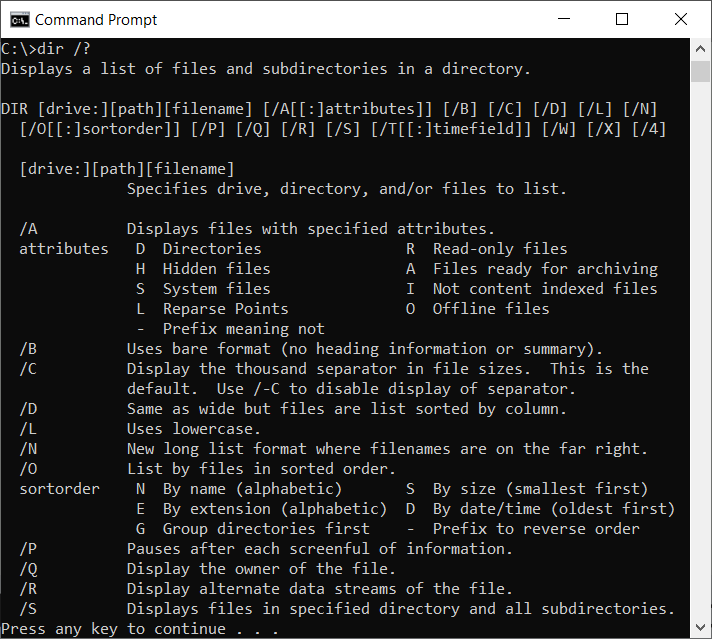
\includegraphics[width=\linewidth]{runtime-parameters-win10-cmd-dir}

		Description of configuration options
	\mynextcolumn
		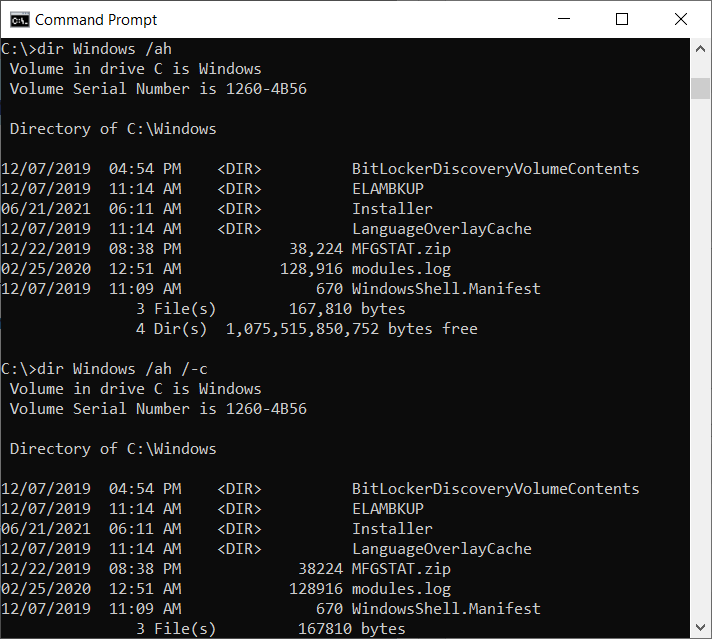
\includegraphics[width=\linewidth]{runtime-parameters-win10-cmd-dir2}

		Two different instances? \pause\pause separator \emph{,} in file sizes
	\end{mycolumns}
\end{frame}

\subsection{Preference Dialogs}

\begin{frame}{Example: Preference Dialogs}
	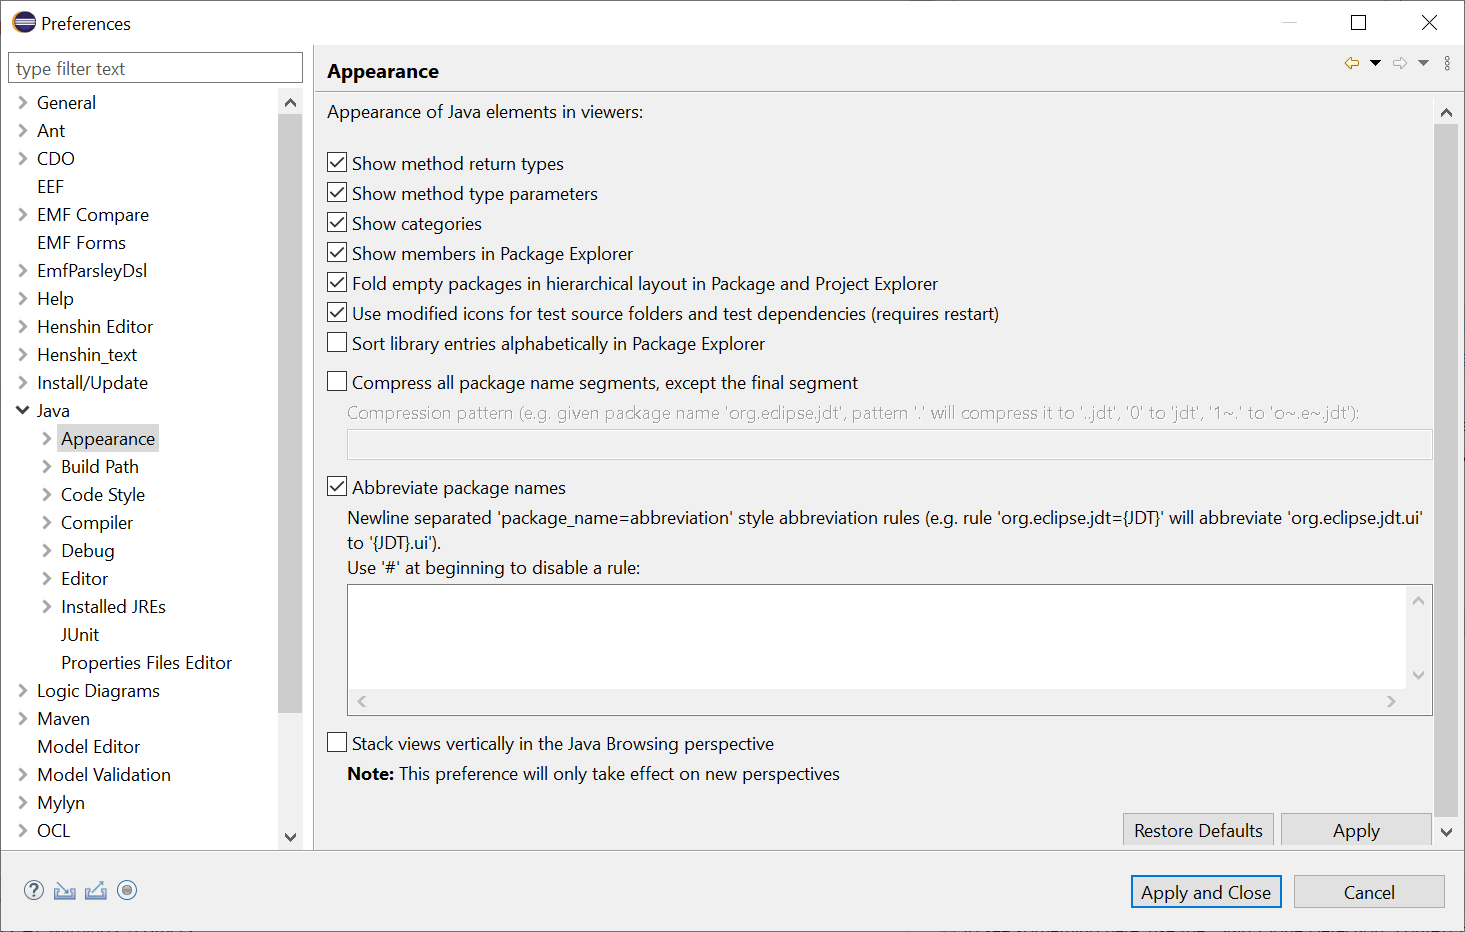
\includegraphics[width=0.75\linewidth]{preferences-eclipse}
\end{frame}

\subsection{Configuration Files}

\begin{frame}{Example: Configuration Files}
	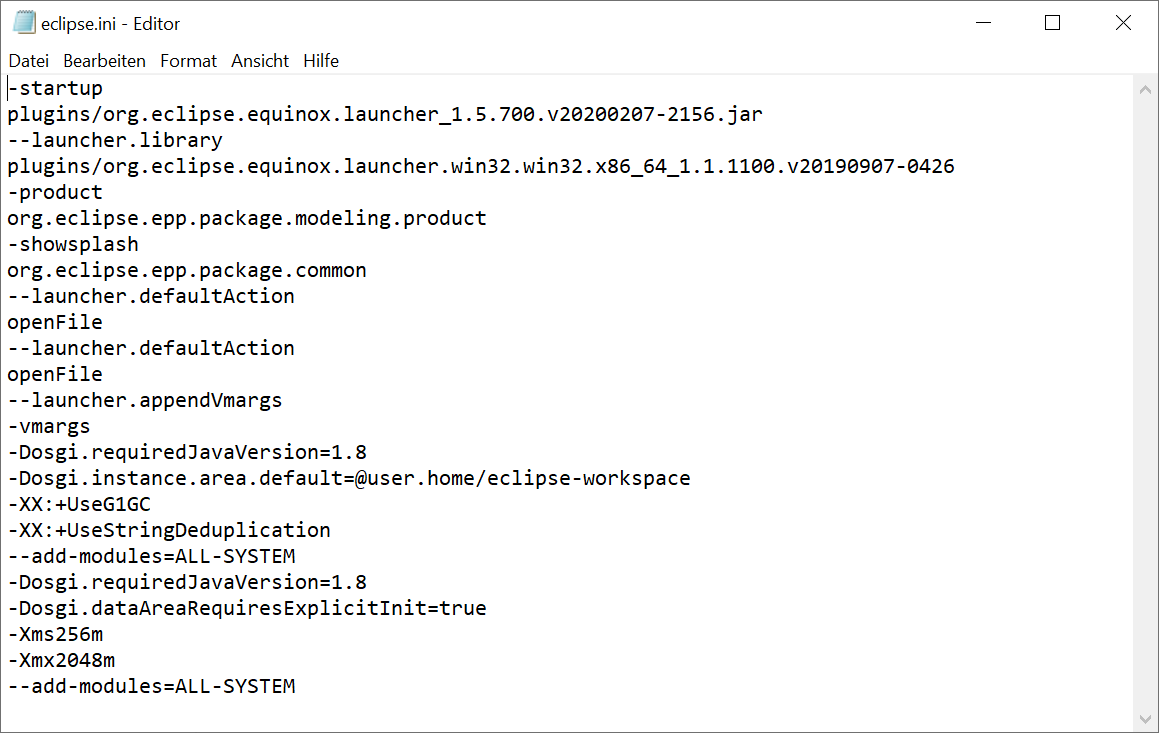
\includegraphics[width=0.75\linewidth]{configfile-eclipse-ini} % das sind ja eigentlich auch nur CLI options - besser eine richtige INI Datei?
\end{frame}

\subsection{Runtime Variability}

\begin{frame}{What do these examples have in common?}
	\begin{mycolumns}[columns=3,widths={26,36,36},animation=none]
		\pic[width=\linewidth]{runtime-parameters-win10-cmd-dir}
	\mynextcolumn
		\pic[width=\linewidth]{preferences-eclipse}
	\mynextcolumn
		\pic[width=\linewidth]{configfile-eclipse-ini}
	\end{mycolumns}
		
	\uncover<2->{
		\begin{mycolumns}[widths={57},animation=none]
			\mynote{Configuration Options}{
				\begin{itemize}
					\item Behavior of a program is determined by configuration options being interpreted at runtime
					\item Choices offered by variability are decided at runtime
					\item Configuration may happen interactively (command-line parameters, preference dialogs) or non-interactively (configuration files)
				\end{itemize}
			}			
		\mynextcolumn	
			\mydefinition{Runtime Variability\mysource{\fospl\mypage{49}}}{
				Runtime variability \deutsch{Laufzeitvariabilität} is decided after compilation when the program is started (aka. load-time variability) or during program execution.
			}	
		\end{mycolumns}
	}
\end{frame}

\subsection{Configuration Options}

\xkcdframe{2694}

\begin{frame}{Example: Graph Library}
	A simple library for graphs providing \ldots\\~\\
	\begin{mycolumns}[t]
		\myexample{\ldots\ Data Structures}{
			\begin{itemize}
				\item Directed/undirected edges
				\item Weighted/unweighted edges 
				\item Colored/uncolored nodes
				\item \ldots
			\end{itemize}
		}		
	\mynextcolumn
		\myexample{\ldots\ and Algorithms}{
			\begin{itemize}
				\item Vertex numbering
				\item Vertex coloring 
				\item Shortest path
				\item Minimum spanning tree 
				\item \ldots
			\end{itemize}
		}
	\end{mycolumns}
\end{frame}

\begin{frame}{Features of a Graph}
	\begin{mycolumns}[t,columns=4]
		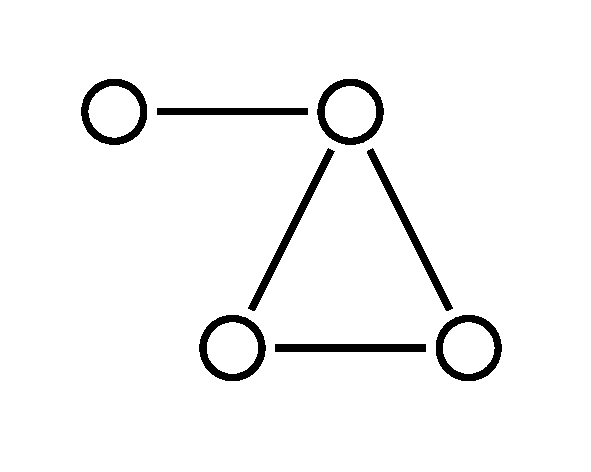
\includegraphics[width=\linewidth,page=1]{graphs}
		\includegraphics[width=\linewidth,page=3]{graphs}
		\centering\Huge\vdots
	\mynextcolumn
		\includegraphics[width=\linewidth,page=5]{graphs}
		\includegraphics[width=\linewidth,page=7]{graphs}
		\centering\Huge\vdots
	\mynextcolumn
		\includegraphics[width=\linewidth,page=11]{graphs}
		\includegraphics[width=\linewidth,page=13]{graphs}
		\centering\Huge\vdots
	\mynextcolumn
		\includegraphics[width=\linewidth,page=15]{graphs}
		\includegraphics[width=\linewidth,page=17]{graphs}		
		\centering\Huge\vdots
	\end{mycolumns}
\end{frame}

\begin{frame}{Features as Configuration Options}
	\begin{mycolumns}[columns=3,widths={25,25},animation=none]
		\myexampletight{Directed}{\includegraphics[width=\linewidth,page=3]{graphs}}
		\myexampletight{Colored}{\includegraphics[width=\linewidth,page=11]{graphs}}
	\mynextcolumn
		\myexampletight{Weighted}{\includegraphics[width=\linewidth,page=5]{graphs}}
		\myexampletight{Weighted, Colored}{\includegraphics[width=\linewidth,page=15]{graphs}}
	\mynextcolumn
		\pause\includegraphics[width=0.45\linewidth,page=6]{graphs}
		\hfill
		\includegraphics[width=0.45\linewidth,page=12]{graphs}
		
		~\pause
		
		\mynote{Configuration of Graph Data Structures}{
			\begin{itemize}
				\item Typically, configuration options are \emph{flags}
				\item Their boolean value determines which features are \emph{activated} / \emph{deactivated}
			\end{itemize}
		}
	\end{mycolumns}
\end{frame}

\subsection{Valid Combinations of Options}

\begin{frame}{\myframetitle}
	\begin{mycolumns}[columns=4,widths={65,5,15,15},animation=none]
		\begin{tabular}{llll}
			\toprule
			{\bf Algorithm} 							& {\bf Graph type} 	& {\bf Weights} & {\bf Coloring}  \\ \midrule
			{\em Vertex numbering}			  & *          				& *        			& *         			\\
			{\em Vertex coloring}       	& undirected 				& *        			& colored   			\\
			{\em Shortest path}        		& directed   				& weighted 			& *         			\\
			{\em Minimum spanning tree} 	& undirected 				& weighted 			& *         			\\
			\ldots         					& \ldots 			 			& \ldots 		  	& \ldots 					\\ \bottomrule
		\end{tabular}
		\vspace{5mm}	
		\uncover<2->{\begin{note}{Dependencies Between Features Must Be Checked}
			\begin{itemize}
				\item when configuration options are loaded at startup
				\item whenever options are loaded/changed at runtime
			\end{itemize}
		\end{note}}
	\mynextcolumn
	\mynextcolumn
		\myexampletight{Directed\\~}{\includegraphics[width=\linewidth,page=3]{graphs}}	
		\myexampletight{Colored\\~}{\includegraphics[width=\linewidth,page=11]{graphs}}	
	\mynextcolumn
		\myexampletight{Weighted\\~}{\includegraphics[width=\linewidth,page=5]{graphs}}	
		\myexampletight{Weighted,\\Colored}{\includegraphics[width=\linewidth,page=15]{graphs}}
	\end{mycolumns}
\end{frame}